
\section{Richiami di termodinamica}

Nel caso di flusso incomprimibile si può avere un condotto a sezione variabile
per variare la velocità del flusso si possono usare condotti acceleranti
(ugelli) o deceleranti (diffusori).

Rallentando l'acqua in uscita dalla turbina si recupera l'energia cinetica
residua del flusso.

Il condotto è qualsiasi sezione di passaggio del fluido, non necessariamente un
``tubo'', come ad esempio lo spazio tra le palette della turbina.

In un motore a 4 tempi si ha una condizione di ``incrocio'' in cui entrambe le
valvole sono aperte.

Il lavoro è ritenuto positivo quando ``esce'' dal sistema mentre è negativo
quando il lavoro sulla macchina viene eseguito al sistema.

\subsection{Trasformazione reversibile}
Si parla di trasformazione reversibile se non si ha variazione di entropia,
ossia se non rimane alcuna traccia della trasformazione.
Se c'è produzione entropica stai degradando il lavoro.

Rendimento politropico(?)

$$
h = q+pv
$$

Sistemi chiusi, il lavoro è funzione della variazione di volume $pdv$
\begin{equation}
u_B - u_A = Q - L = \int_{s_A}^{s_B} Tds - \int_{v_A}^{v_B}pdv
\end{equation}

Sistemi aperti, il lavoro è funzione della variazione di pressione $vdp$
\begin{equation}
h_B - h_A = Q - L =  \int_{s_A}^{s_B} Tds + \int_{p_A}^{p_B} vdp
\end{equation}

In un compressore ad esempio si ha l'area sottesa al piano h-s il lavoro
d'attrito, nella parte superiore invece il lavoro di controrecupero.

\begin{figure}[h]
\centering
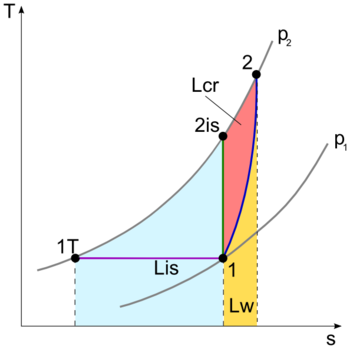
\includegraphics[width=0.4\linewidth]{compressione}
\end{figure}

Si parla di piano termodinamico del lavoro quello P-v,

Uno scambiatore di calore non prevede lavoro meccanico, non ha parti in
movimento..
Il termine $vdp$ si annulla a causa della pressione costante, quindi non c'è
lavoro mentre l'integrale $TdS$ mostra il lavoro fornito.
Innalzando la temperatura media di adduzione e sottrazione del ciclo si aumenta
il rendimento di Carnot.
$$
\eta_g = \eta_c\eta_r\eta_mm
$$
il termine critico è il rendimento reale $\eta_r$, il ciclo combinato è quello
con strategia per aumentare il pi¡u possibile le differenze di temperatura.

Solo per i \textit{processi reversibili} si ha l'uguaglianza tra l'incremento
di entropia e il prodotto $dQ$ e $1/T$, considerando una temperatura media
infatti
$$
s_B - s_A = \frac{\int_A^B \delta Q}{T_m} = \frac{Q}{t_m}
$$
Rendimento di Carnot:
\begin{equation}
\eta = \frac{Q_1-Q_2}{Q_1} = ... = 1 - \frac{T_{ms}}{T_ma}
\end{equation}


Al limite si desidera un rendimento unitario.

\subsection{Cause di irreversibilità}
SI prenda in esempio uno scambiatore a flussi
sparati.
Ci sarà sempre un limmite di ingombro, dunque non tutto il calore può passare
del fulolso caldo e non per lo scambiatore caldo.
La produzione entropica aumenta all'aumentare delle distanze tra le
temperature.
Non si superano di solito gli 8 spilllamenti per gli scambiato fa vatto.

Lavoro di attrito
In un condotto si ail...


In un impianto a vapore si ha una sottrazione di calore a temperatura costante
e a d un valore di calroad'acqua staavvenend.
%Inserisci foto ciclo HIRN
L'adduzione del calore avviene ad una temperatura relativamente bassa.

La caldaia a vapore è composta in tre parti
Economizzatore, vaporizzatore, surriscaldatore.

Spillando vapore dalla turbina psi piö otitmizzare la temperature in ingresso,
ovvero avere acqua in ingresso al generatore di vapore con una teoirad iche tii.

La potenza in un impianto vapore si scrive con
$$
P = \dot{m}_{VAP}\cdot\Delta h\cdot\eta_{m}
$$

Il salto entalpico è quello che massimizza il rendimento.



Nella realtà non c'è mai una trasformazione isobara in camera di combustione,
esistono delle piccole cadute di pressione in camera di combustione.

Con la rigenerazione si spilla vapore dalla turbina, cambia l'integrale Tds del
ciclo, partendo da una temperatura iniziale più alta si risparmia calore,
ovvero si risparmia combustibile, pari a
$$
\Delta Q_1 = \eta_b\Delta \dot{m}_f H_i
$$

Gli spillamenti non possono mai essere completamente chiusi, la turbina è
costruire per possedere una certa quantità di spillamenti, è disegnata per
contenere una certa portata d'acqua, si può sostituire lo scambiatore di
recupero con un impianto solare ad esempio.


La generazione entropica in uno scambiatore è legata alle differenze di
temperature per il lorop prodotto.
La produzione entropica distrugge l'exergia.

Vanno inseriti più spillamenti e più scambiatori di calore per ridurre le
irreversibilità.


